\subsubsection{Adam: Adaptive Moment Estimation}
\label{sec:training-adam}
Learning rate schedules have the problems of defining their parameters in advance and applying the same learning rate to every weight and bias.
Hence, the RMSProp (Root Mean Square Propagation) optimizer was developed\cite{Tieleman2012}.
Its objective is illustrated in \figref{fig:rmsprop}.
The ellipses represent contour lines.
The orange line visualizes the process of gradient descent.
Using it can result in parameters oscillating in one direction while making progress in another one moving to the minimum.
The objective of RMSProp, represented by the blue line, tries to dampen the oscillations by slowing down learning of the responsible parameter and fasten up the other one.
Hence, it can use a larger learning rate and reaches the minimum more quickly.
\begin{figure}
	\centering
	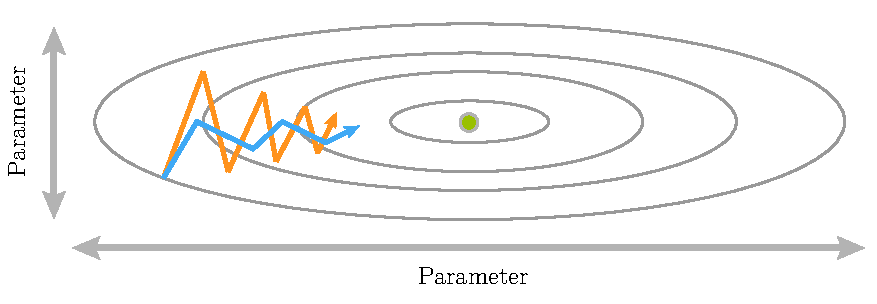
\includegraphics[]{images/rmsprop.pdf}
	\caption[Process of Gradient Descent and RMSProp]{Process of gradient descent and RMSProp using contour lines. The orange line illustrates the process of gradient descent. It oscillates and moves slowly to the minimum. The blue line shows the process of the RMSProp algorithm. While one parameter changes slower the other one changes faster. Hence, it dampens oscillations and moves faster to the minimum.}
	\label{fig:rmsprop}
\end{figure}
RMSProp adapts a learning rate to each of the parameters.
Furthermore, it divides the learning rate for a parameter by a weighted running average of the magnitudes of its previous gradients.
The weighted running average is calculated by
\begin{subequations}
	\label{eq:adam-second-momentum}
	\begin{align}
		v(w^{[l]}_{jk}, \tau) &= \beta_2 v(w^{[l]}_{jk}, \tau - 1) + (1-\beta_2) (\nabla \vec{J}(w^{[l]}_{jk}))^2 \\
		v(b^{[l]}_{j}, \tau) &= \beta_2 v(b^{[l]}_{j}, \tau - 1) + (1-\beta_2) (\nabla \vec{J}(b^{[l]}_{j}))^2
	\end{align}
\end{subequations}
where hyperparameter $\beta_2$ is the forgetting factor.
As a value its author suggests $\beta_2 = 0.9$.
The subscript $2$ is for later purposes and could be omitted for now.
The squaring operation is done element-wise.
So this expression adds kind of an inertia to the update procedure dampening oscillations and building up speed on flat surfaces.
Finally, the parameters are updated by
\begin{subequations}
	\begin{align}
		w^{[l]}_{jk} &:= w^{[l]}_{jk} - \frac{\gamma}{\sqrt{v(w^{[l]}_{jk}, \tau)}} \nabla \vec{J}(w^{[l]}_{jk}) \\
		b^{[l]}_{j} &:= b^{[l]}_{j} - \frac{\gamma}{\sqrt{v(b^{[l]}_{j}, \tau)}} \nabla \vec{J}(b^{[l]}_{j})
	\end{align}
\end{subequations}
using the weighted moving average just calculated.
Let's say the horizontal parameter is $w_1$ and the vertical one $w_2$ referring to \figref{fig:rmsprop}.
Due to the oscillations the gradient $\nabla \vec{J}(w_2)$ is much larger than $\nabla \vec{J}(w_1)$.
Hence, $v_2$ is larger than $v_1$ resulting in a smaller update for $w_2$ and a larger one for $w_1$.
This yields a more direct moving to the minimum.
However, this approach does not make it easier to configure the learning rate as the step size is independent of it.
Though, it improves the speed of the optimization process because a better set of weights is discovered in fewer training steps than with pure gradient descent.
The Adam (Adaptive Moment Estimation) optimization is an update to the RMSProp algorithm by adding a momentum
\begin{subequations}
	\label{eq:adam-first-momentum}
	\begin{align}
		m(w^{[l]}_{jk},\tau) &= \beta_1 m(\tau -1) + (1- \beta_1) \frac{\partial J}{\partial w^{[l]}_{jk}} \\
		m(b^{[l]}_{j},\tau) &= \beta_1 m(\tau -1) + (1- \beta_1) \frac{\partial J}{\partial b^{[l]}_{j}}
	\end{align}
\end{subequations}
for each parameter using a weighted average of latest gradients\cite{DBLP:journals/corr/KingmaB14} where $\beta_1$ is the forgetting factor.
This momentum can be imagined as a ball in a bowl-shaped cost function rolling downwards and building up speed depending on the gradients.
The hyperparameter $\beta_1$ represents friction.
This approach can be summarized by using running averages of both the gradients and the second moments of the gradients.
Due to the initialization $\vec{v} = \vec{0}$ and $\vec{m} = \vec{0}$ these values are biased towards zero, especially during the first few iterations.
A correction is desirable, because the first and second moments are only estimations.
In general, an estimation should equal the parameter that is tried to be estimated.
Hence, the property
\begin{subequations}
	\begin{align}
		E[m] &= E[g]\\
		E[v] &= E[g^2]
	\end{align}
\end{subequations}
needs to be fulfilled, where $E[\cdot]$ represents the expectation of a variable.
These properties only hold true, if unbiased estimators are used.
Hence, the corrected values are expressed by
\begin{subequations}
	\label{eq:adam-corrected}
	\begin{align}
	\hat{m}(w^{[l]}_{jk}, \tau) &= \frac{m(w^{[l]}_{jk},\tau)}{1-\beta_1^\tau} \\
	\hat{m}(b^{[l]}_{j}, \tau) &= \frac{m(b^{[l]}_{j},\tau)}{1-\beta_1^\tau} \\
	\hat{v}(w^{[l]}_{jk}, \tau) &= \frac{v(w^{[l]}_{jk}, \tau)}{1-\beta_2^\tau} \\
	\hat{v}(b^{[l]}_{j}, \tau) &= \frac{v(b^{[l]}_{j}, \tau)}{1-\beta_2^\tau}
	\end{align}
\end{subequations}
using the expression from before.
Finally,
\begin{subequations}
	\label{eq:adam-update}
	\begin{align}
		w^{[l]}_{jk} := w^{[l]}_{jk}-\gamma \frac{\hat{m}(w^{[l]}_{jk})}{\sqrt{\hat{v}(w^{[l]}_{jk})} + \epsilon} \\
		b^{[l]}_{j} := b^{[l]}_{j}-\gamma \frac{\hat{m}(b^{[l]}_{j})}{\sqrt{\hat{v}(b^{[l]}_{j})} + \epsilon}
	\end{align}
\end{subequations}
updates the parameters, where $\epsilon$ is a small constant for preventing a division by zero.
As for other optimization algorithms the learning rate $\gamma$ needs to be tuned.
The remaining hyperparameters are recommended by \textit{Kingma et al.} to be $\beta_1 = 0.9$, $\beta_2 = 0.999$ and $\epsilon = 10^{-8}$.
However, the latter has no big impact on the optimization.